%==============================================================================
\chapter{Theoretische Einführung}
\label{sec:theo}
%==============================================================================

\section{Hubbard-Modell}
Das Hubbard-Modell, benannt nach dem britischen Physiker John Hubbard, wird hauptsächlich in der Festkörper-Physik verwendet. Es beschreibt ein Material als Gitter auf dem Teilchen (normalerweise Elektronen) zu einem benachbarten Gitter-Punkt springen können, sofern dabei das Pauli-Prinzip nicht verletzt wird und sich nur gegenseitig abstoßen Wenn sie sich auf der selben Position im Gitter befinden. In \ref{fig:pic2} wird dieses Gitter für den zweidimensionalen Fall schematisch gezeigt. Die Berücksichtigung der Abstoßung unterscheidet, dass Hubbard-Modell von einigen anderen Modellen und ermöglicht ihm, beispielsweise den Übergang zwischen Leiter und Isolator in bestimmten Metall-Oxiden zu beschreiben. Der Hamilton-Operator dieses Modells sieht wie folgt aus \cite{Hubbard}:
\begin{equation}\label{Hubbard_original}
H = \sum_{i,j}\sum_{\sigma}T_{ij} c_{i\sigma}^\dag c_{j\sigma} + \frac{I}{2} \sum_{i}n_{i\uparrow}n_{i\downarrow} - \frac{I}{2}Nn^2
\end{equation}
Hier ist $ c^\dag $ der Erzeugungs-Operator, $ c $ der Vernichtungs-Operator und $ n = c^\dag c $ der Besetzungszahl-Operator. Der Sprung von einem Platz zu einem Anderen wird als Vernichtung des Teilchens auf der Ursprungsposition und der Erzeugung auf der Zielposition beschrieben. Der Parameter I steht für die Potentielle Energie aufgrund der Coulomb-Abstoßung. Das Matrixelement $ T_{ij} $ gibt die kinetische Energie eines Elektrons beim Sprung von Gitterpunkt $ i $ zu Gitterpunkt $ j $ an und ist abhängig vom Überlapp der beiden Orbitale. Zusätzlich zu der Annahme, dass die Abstoßenden Kräfte nur zwischen Elektronen auf dem selben Platz wirken, wird angenommen, dass Elektronen nur zu ihrem nächsten Nachbarn springen, dies bedeutet für ein homogenes Gitter $ T_{ij} \approx -t\delta_{\langle ij \rangle} $\cite{schoett2014}. Durch diese Vereinfachung muss nun nicht mehr das Matrixelement für jede Kombination aus zwei Gitterplätzen berechnet werden, sondern nur noch für direkte Nachbarn, wodurch die Matrix deutlich dünner besetzt wird. Zusammen mit dem Parameterwechsel $ U = \frac{I}{2} $ und dem Weglassen der Konstante führt dies zu einer einfacheren Form des Hamilton-Operators \cite{Rickayzen,schoett2014}:
\begin{equation}\label{Hubbard_standard}
H = \underbrace{-t\sum_{\langle ij\rangle,\sigma}\left( c_{i\sigma}^\dag c_{j\sigma} + c_{j\sigma}^\dag c_{i\sigma}\right)}_{\substack{H_0}}  + \underbrace{U \sum_{i}n_{i\uparrow}n_{i\downarrow}}_{\substack{H_I}}
\end{equation}
Die Bedeutung der beiden Parameter $ t $ und $ U $ wird in \ref{fig:pic1} verdeutlicht mit $ t $ als Tunnelenergie und $ U $ als Potentielle Energie zweier Elektronen auf dem selben Gitterplatz.
$ H_I $ ist der Abstoßungsterm des Hamilton-Operators und $ H_0 $ der Hopping-Term.
Der nicht interagierende Term $ H_0 $ lässt sich durch eine Fourier-Transformation in den Impulsraum diagonalisieren \cite{schoett2014}
\begin{equation}\label{Hubbard_momentum}
H = \sum_{\boldsymbol{k} \sigma} \epsilon_{\boldsymbol{k}} c_{\boldsymbol{k}\sigma}^\dag c_{\boldsymbol{k}\sigma}\\
\end{equation}
$ \epsilon_{\boldsymbol{k}} $ ist die Dispersion der Elektronen. Die Erzeugungs- und Vernichtungsoperatoren wirken nun nicht mehr auf zwei verschiedene Gitter Plätze sondern das Elektron mit dem Impuls $ \boldsymbol{k} $. Sie können einfach als Wannier-Funktion
\begin{equation}\label{Wannier}
\psi_{\boldsymbol{k}} \left( \boldsymbol{x}\right) = \frac{1}{\sqrt{N}}\sum_{j} e^{i\boldsymbol{k}\boldsymbol{R}_j} \phi(\boldsymbol{x}-\boldsymbol{R}_j)
\end{equation} 
der lokalen Operatoren berechnet werden
\begin{equation}\label{c_momentum}
c_{\boldsymbol{k}\sigma} = \frac{1}{\sqrt{N}}\sum_{j} e^{i\boldsymbol{k}\boldsymbol{R}_j} c_{j\sigma}, \qquad c_{\boldsymbol{k}\sigma}^\dagger = \frac{1}{\sqrt{N}}\sum_{j} e^{-i\boldsymbol{k}\boldsymbol{R}_j} c_{j\sigma}^\dagger
\end{equation}\cite{Hubbard}  
Durch Einsetzen dieser in \eqref{Hubbard_momentum} erhält man für $ T_{ij} $ aus \eqref{Hubbard_original}
\begin{equation}\label{T}
T_{jl} = \frac{1}{N} \sum_{\boldsymbol{k}}\epsilon_{\boldsymbol{k}} e^{i\boldsymbol{k}\left( \boldsymbol{R}_j - \boldsymbol{R}_l\right) }
\end{equation}

\begin{figure}[h!]
	\begin{subfigure}{.5 \textwidth}
		\centering
		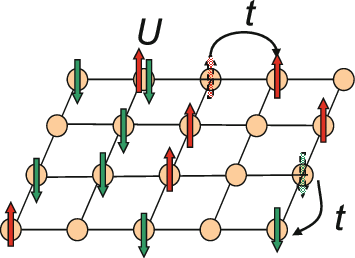
\includegraphics[width=0.8\linewidth]{../figs/graphics/pic2}
		\caption{\cite{FigHubbardModel2}}
		\label{fig:pic2}
	\end{subfigure}
	\begin{subfigure}{.5 \textwidth}
		\centering
		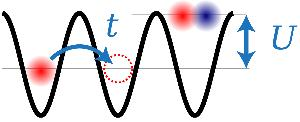
\includegraphics[width=0.8\linewidth]{../figs/graphics/pic1}
		\caption{\cite{FigHubbardModel1}}
		\label{fig:pic1}
	\end{subfigure}
\caption[Veranschaulichung des Hubbard-Modells]{(a): Hier sieht man ein zweidimensionales quadratisches Gitter, die orangen Punkte symbolisieren Atome mit jeweils einem freien Orbital und die Gitterlinien zeigen die erlaubten Sprünge der Elektronen (hier als Pfeile dargestellt)\\(b): Diese Abbildung zeigt das Potential eines eindimensionalen Atom-Gitters, der Parameter t steht für die kinetische Energie eines Elektrons (rote und blaue Punkte) beim Sprung zu Nachbaratom, der Parameter U steht für die Potentielle Energie zweier Elektronen (up \& down) die sich gegenseitig abstoßen.}
\label{HubbardFigs}
\end{figure}


\subsection{Vereinfachende Eigenschaften}
Wie man der Definition des Hamilton-Operators \eqref{Hubbard_standard} entnehmen kann bleiben die Teilchenzahl $ \hat{N} $, der gesamt Spin $ \hat{S}^2 $ und die Z-Komponente des Spins $ \hat{S}_z $ bei der Anwendung des Hamilton-Operators erhalten. Das führt dazu, dass die Matrix des Operators (bei geeigneter Wahl der Basis) aus Blockmatrizen für feste $ N $ entlang der Diagonalen besteht, welche wiederum den selben Aufbau mit Blöcken für feste $ S_z $ haben. Diese Eigenschaft ermöglicht es die Basis zu unterteilen, sodass man sich auf die wichtigsten Zustände beschränken kann. Es ist beispielsweise sehr unwahrscheinlich, dass alle Spins in dieselbe Richtung zeigen. Der interessanteste Block ist der mit halber Füllung und neutraler Spin-Ausrichtung, da dieser über die meisten Zustände verfügt und außerdem den Grundzustand enthält.

Eine weitere Eigenschaft, die man sich zu Nutze machen kann ist die Translations-Invarianz. Wenn man ein Gitter mit periodischen Grenzen betrachtet, also den Elektronen am Ende des Gitters erlaubt direkt zum gegenüberliegenden Ende zu springen, sollte klar sein, dass eine Translation aller Elektronen in eine Richtung nichts an den Physikalischen Eigenschaften des Zustandes ändert, da nur die Anordnung der Elektronen für diese verantwortlich ist, der Hamilton-Operator ist unabhängig von den Positionen einzelner Elektronen. Daraus folgt, dass einige der Basiszustände äquivalent sind und sich als Translation eines anderen Zustands schreiben lassen. Der Translationsoperator $ T $ verschiebt alle Elektronen um einen Gitterplatz. Nach einem kompletten Durchgang ist man wieder am Anfangszustand angekommen $ T^N\ket{a} = \ket{a} $. Da die verschiedenen Translationen äquivalent sind, gilt auch für die Eigenwerte von $ T $: $ \lambda^N = 1 $, daraus folgt $ \lambda = e^{ik} $ mit $ k = m\frac{2\pi}{N} $ für $ m \in \mathbb{N}, m < N $. Um diese Kriterien zu erfüllen wird der Impuls-Zustand $ \ket{a(k)} $ als 
\begin{equation}\label{momentumstate}
\ket{a(k)} = \frac{1}{\sqrt{N_a}}\sum_{r=0}^{N-1}e^{-ikr}T^r\ket{a}
\end{equation}
definiert, sodass $ T\ket{a(k)} = e^{ik}\ket{a(k)}$ gilt, wobei $ \ket{a} $ ein Referenzzustand aus der lokalen Basis ist und $ N_a $ für die Normierung sorgt \cite{Sandvik}. Der Startzustand wird in einigen Fällen schon vor $ N $ Verschiebungen wieder erreicht, dadurch werden die möglichen $ k $ eingeschränkt und die Normierung muss beachtet werden. Dazu wird $ R_a $ als kleinst mögliche Lösung von $ T^{R_a}\ket{a} = \ket{a} $ gewählt. Dann gilt
\begin{equation}\label{k}
k = m\frac{2\pi}{R_a},\qquad m \in \mathbb{N},\: m < R_a
\end{equation}
und
\begin{equation}\label{N_a}
N_a = \frac{N^2}{R_a}.
\end{equation}
Der Vorteil dieser Basis ist, dass der Hamilton-Operator in noch kleinere Blöcke mit konstantem $ k $ aufgeteilt werden kann, da dieses ebenfalls erhalten ist.

\subsection{Analytische Lösung für den Grundzustand}
Der Grundzustand des Hubbard-Modells, ist für diese Arbeit von großer Bedeutung, da im Photoemmissions- und -absorptionsspektrum die Energiedifferenz eines Zustandes zum Grundzustand auf der x-Achse aufgetragen wird und die Grundzustandsenergie somit in jedem Eintrag steckt. Da die direkte Lösung des Hubbard-Modells sogar im eindimensionalen Fall schon auf sehr kleine Gitter beschränkt ist wird die Grundzustandsenergie nicht mit den realen Eigenschaften des Materials übereinstimmen, jedoch kann man eine Konvergenz mit steigender Gitterlänge gegen diese analytische Lösung erwarten
\begin{equation}\label{analytisch}
E_0(U)=-4L\int_{0}^{\infty}\frac{J_0(\omega)J_1(\omega)}{\omega\left( 1+\exp\left( \omega\frac{U}{2}\right) \right) }d\omega
\end{equation}\cite{Monien}
Hier steht $ L $ für die Anzahl der Gitterplätze und $ J_n(\omega) $ für die Besselfunktion erster Gattung.



\section{Spektralfunktion}
Spektralfunktionen werden in der Physik genutzt um die physikalischen Eigenschaften (z.B. die Zustandsdichte) eines Materials darzustellen.\cite{Lin} Das Ergebnis hat die Form eines Spektrums, wie man es auch experimentell aufnehmen kann, daher eignet sich die Spektralfunktion gut um eine Theorie mit tatsächlichen Messwerten zu vergleichen.
Sobald man die Greensche Funktion kennt, kann ihre Spektralfunktion wie folgt bestimmt werden
\begin{equation}\label{G2A}
A(\omega)= \lim\limits_{\eta \rightarrow 0}\,-\frac{1}{\pi}\Im\left[ G(\omega+i\eta)\right] 
\end{equation}
Um aus einer Spektralfunktion ihre Greensche Funktion zu extrahieren muss man eine Hilberttransformation anwenden
\begin{equation}\label{A2G}
G(z) = \int_{-\infty}^{\infty}\frac{A(\zeta)}{z- \zeta}\dd{\zeta}
\end{equation}
\cite{Rickayzen,schoett2014}
Eine Spektralfunktion kann als Summe von Deltafunktionen geschrieben werden, deren Gewichtung vom Matrixelement zwischen dem gestörten Grundzustand $ B\ket{\psi_0} $ und dem angeregten Zustand $ \ket{\psi_m} $ gegeben ist.
\begin{equation}\label{deltasum}
A(\omega) =\sum_{m}\abs{\bra{\psi_m}B\ket{\psi_0}}^2\delta\left( \omega-(\lambda_m-\lambda_0)\right) 
\end{equation}
Die kombinierte Spektralfunktion aus Photoemission und Photoabsorption, welche der Zustandsdichte entspricht wenn beide Operatoren auf das selbe Elektron wirken, verwendet als Störoperator $ B $ den Erzeugungs- und Vernichtungsoperator. Man erhält für diese also folgende Formel
\begin{equation}\label{rho}
\rho(\omega) = \sum_{m}\abs{\bra{\psi_m}c^\dagger_i\ket{\psi_0}}^2\delta\left( \omega -\lambda_m +\lambda_0\right) + \sum_{n}\abs{\bra{\psi_n}c_i\ket{\psi_0}}^2\delta\left( \omega +\lambda_n + \lambda_0\right)
\end{equation}

\section{Greensche Funktion}
Die Greensche Funktion kann allgemein zur Lösung von Differentialgleichungen genutzt werden, indem sie für einen bestimmten linearen Differentialoperator $ L $ die Deltafunktion ergibt
\begin{equation}\label{G1}
LG(x,y) = \delta(x-y)
\end{equation}
Dies ermöglicht es, sozusagen das Inverse des Differentialoperators zu berechnen. Wenn $ L f(x) = g(x) $ gilt und sowohl $ L $ als auch $ g(x) $ bekannt sind, ist es dennoch nicht trivial $ f(x) $ zu bestimmen, da man den Operator nicht einfach invertieren kann. Mit der Greenschen Funktion kann dies durch folgenden \emph{Trick} dennoch gelingen
\begin{align*}
L f(x) &= g(x)\\
L f(x) &= \int \delta(x-y)g(y)\dd{y}\\
L f(x) &= \int L G(x,y)g(y)\dd{y}\\
\end{align*}
\begin{equation}\label{Hilbert}
\Rightarrow f(x)  = \int G(x,y) g(y) \dd{y}
\end{equation}
In der Physik der kondensierten Materie haben Greensche Funktionen häufig nur noch wenig Ähnlichkeiten mit ihrer ursprünglichen mathematischen Definition.
In \eqref{G2A} wird die Spektralfunktion aus der Greenschen Funktion erstellt. Wie man in \eqref{deltasum} sieht lässt sich die Spektralfunktion als Summe aus Deltafunktionen darstellen, beim Vergleich mit \eqref{G1} stellt man also fest, dass $ \lim\limits_{\eta \rightarrow 0}\,-\frac{1}{\pi}\Im $ als Operator $ L $ infrage kommt (zusätzlich muss natürlich $ i\eta $ zu $ \omega $ hinzu addiert werden). Unter den verschiedenen Darstellungen der Deltafunktion befindet sich auch 
\begin{equation}\label{delta}
\delta(x - y) =\lim\limits_{\eta \rightarrow 0}\,-\frac{1}{\pi}\Im\left[ \frac{1}{x - y +i\eta}\right] 
\end{equation}
wodurch klar ist, dass
\begin{equation}\label{G}
G(x,y) = \frac{1}{x - y}
\end{equation}
gilt. Diese kann einfach mit \eqref{rho} in \eqref{Hilbert} eingesetzt werden und man erhält die Greensche Funktion für die Zustandsdichte
\begin{equation}\label{Grho}
G(\omega) = G_{ii}(\omega) = \frac{\sum_{m}\abs{\bra{\psi_m}c^\dagger_i\ket{\psi_0}}^2}{\omega +\lambda_0 -\lambda_m } + \frac{\sum_{n}\abs{\bra{\psi_n}c_i\ket{\psi_0}}^2}{\omega + \lambda_0 +\lambda_n}
\end{equation}
%\begin{equation}\label{TAB}
%G(\boldsymbol{r}_1,\tau_1,\boldsymbol{r}_2,\tau_2) = \left\langle T\,A(\boldsymbol{r}_1,\tau_1)B(\boldsymbol{r}_2,\tau_2)\right\rangle 
%\end{equation}
%Hier ist $ T $ der Zeitordnungsoperator und $ A $ und $ B $ sind beliebige Quantenmechanische Operatoren. Der Einfachheit halber wird in dieser Arbeit von hier an die Greensche Funktion für das Photoemmissions- und -absorptionsspektrum bei $ T = \SI{0}{\kelvin} $ behandelt, da man in der Regel an dieser interessiert ist. Für diese Greensche Funktion wählt man $ c_i(\tau) $ und $ c_j^\dagger(0) $ als Operatoren.
%\begin{align*}
%G_{ij}(\tau) &= \left\langle T\,c_i(\tau)c_j^\dagger(0)\right\rangle \\
% &= \Theta(\tau)\bra{0}c_i(\tau)c_j^\dagger(0)\ket{0} - \Theta(-\tau)\bra{0}c_j^\dagger(0)c_i(\tau)\ket{0}\\
% &= \Theta(\tau)\bra{0}e^{iH\tau}c_ie^{-iH\tau}c_j^\dagger\ket{0} - \Theta(-\tau)\bra{0}c_j^\dagger e^{iH\tau}c_ie^{-iH\tau}\ket{0}\\
% &= \Theta(\tau)\bra{0}c_ie^{-i(H-E_0)\tau}c_j^\dagger\ket{0} - \Theta(-\tau)\bra{0}c_j^\dagger e^{i(H-E_0)\tau}c_i\ket{0}\\
% &= \Theta(\tau)\sum_{m}e^{-i(E_m-E_0)\tau}\bra{0}c_i\ket{m}\bra{m}c_j^\dagger\ket{0} - \Theta(-\tau)\sum_{m}e^{i(E_m-E_0)\tau}\bra{0}c_j^\dagger\ket{m}\bra{m} c_i\ket{0}\\
% &= \sum_{m}e^{-i(E_m-E_0)\abs{\tau}}\left[ \Theta(\tau)\bra{0}c_i\ket{m}\bra{m}c_j^\dagger\ket{0} - \Theta(-\tau)\bra{0}c_j^\dagger\ket{m}\bra{m} c_i\ket{0}\right] \\
%\end{align*}
%Diese Funktion kann nun Fourier-transformiert werden
%\begin{align*}
%	\hat{G}(\omega) &= \int_{-\infty}^{\infty}
%\end{align*}
%\cite{Rickayzen,schoett2014,FZJ2017}
diese lässt sich ebenfalls schreiben als
\begin{equation}\label{GreensFunctionDOS}
G(\omega) = \bra{0}c\frac{1}{(\omega + \lambda_0) I - H}c^\dagger\ket{0} + \bra{0}c^\dagger\frac{1}{(\omega + \lambda_0) I + H}c\ket{0}
\end{equation}\cite{Lu,Stover,Ulm}

\section{Anderson-Impurity-Model}
\begin{equation}\label{key}
H_{A} = \epsilon_d \sum_{\sigma} d_{\sigma}^\dag d_{\sigma} +\sum_{\sigma,l}\epsilon_l c_{l\sigma}^\dag c_{l\sigma} + Un_{d\uparrow}n_{d\downarrow} + \sum_{\sigma,l}\left( V_l c_{l\sigma}^\dag d_{\sigma} + V_l^* d_{\sigma}^\dag c_{l\sigma}\right) 
\end{equation}



\section{DMFT}


\section{Bethe-Gitter}

\section{Lanczos Methode}
Um die Eigenwerte der immer noch zu großen Matrix zu berechnen, kann man die Lanczos Methode verwenden. Diese erzeugt einen invarianten Unterraum der großen Matrix A, bei diesem Unterraum handelt es sich um einen Krylov Unterraum ($b,Ab,A^2b,...,A^{m-1}b$). Der letzte Vektor liegt dabei nicht mehr im Unterraum, aber für ausreichend große m  ist dieser ungefähr proportional zum Vorletzten, da dieser gegen einen Eigenvektor strebt, daher liegt der letzte Vektor näherungsweise auch im Unterraum. Die Lanczos Methode gibt eine tridiagonale Matrix T für diesen Unterraum aus, deren Eigenwerte auch Eigenwerte von A sind.\cite{Lin, FZJ}
\begin{equation}
AQ = QT\;,\;Ty=\lambda y \Rightarrow A(Qy)=\lambda(Qy)
\end{equation} 
In der Regel sind es die größten und kleinsten Eigenwerte von A, die man in Matrix T findet, daher eignet sich die Lanczos Methode um die Energie des Grundzustands, also den kleinsten Eigenwert zu finden. Die Matrix T wird iterativ mit folgender Rekursions-Beziehung gefunden, 
\begin{equation}
Aq_j = \beta_{j-1}q_{j-1}+\alpha_jq_j+\beta_{j}q_{j+1}
\end{equation}
wobei der Vektor $\alpha$ der Hauptdiagonalen und der Vektor $\beta$ den Nebendiagonalen der Matrix T entspricht.\cite{Lloyd}







%%% Local Variables: 
%%% mode: latex
%%% TeX-master: "../mythesis"
%%% End: 